\documentclass[11pt]{article}
\usepackage[utf8]{inputenc}
\usepackage{graphicx}
\usepackage{geometry}
\usepackage{amsmath}
\usepackage{booktabs}
\usepackage{verbatim}
\geometry{margin=1in}
\title{CSE318 Assignment 02\\Solving the MAX-CUT Problem using GRASP}
\author{Gourove Roy \\ Student ID: 2105017}
\date{May 2025}

\begin{document}

\maketitle

\section*{1. Introduction}
The MAX-CUT problem is a classic NP-hard optimization problem. It involves partitioning the vertices of a weighted undirected graph into two subsets such that the total weight of the edges crossing the partition is maximized.

\section*{2. Algorithm Descriptions}

\subsection*{2.1 Randomized Algorithm}
This is the simplest approach where each vertex is randomly assigned to one of two partitions with equal probability. Multiple trials are performed, and the average result is taken to mitigate randomness.

\textbf{Key Characteristics:}
\begin{itemize}
\item Extremely fast but produces low-quality solutions
\item Provides a baseline for comparison
\item No guarantee of solution quality
\end{itemize}

\textbf{High-level Description:}
Given a graph $G = (V, E)$ with weights $w_{uv}$ on edges, each vertex $v \in V$ is randomly assigned to one of the two partitions $X$ or $Y$ with equal probability. The total weight of the cut $(X, Y)$ is:
\[ w(X, Y) = \sum_{u \in X, v \in Y} w_{uv} \]
This process is repeated for a number of iterations, and the average result is recorded.

\textbf{Pseudocode:}
\begin{verbatim}
Input: Graph G = (V, E)
Initialize sets A = {}, B = {}

for each vertex v in V:
    Randomly assign v to A or B

return (A, B)
\end{verbatim}

\subsection*{2.2 Greedy Algorithm}
This deterministic approach builds the solution by always making the locally optimal choice at each step. Vertices are assigned to the partition that maximizes their immediate contribution to the cut.

\textbf{Key Characteristics:}
\begin{itemize}
\item Fast execution with reasonable solutions
\item Prone to getting stuck in local optima
\item No randomness involved
\end{itemize}

\textbf{High-level Description:}
We initialize partitions $X$ and $Y$ using the endpoints of the heaviest edge. For each unassigned vertex $z \in V$, we compute:
\[ w_X(z) = \sum_{y \in Y} w_{zy}, \quad w_Y(z) = \sum_{x \in X} w_{zx} \]
Then we assign $z$ to the partition where it contributes the most to the cut.

\textbf{Pseudocode:}
\begin{verbatim}
Input: Graph G = (V, E)
Initialize sets A = {}, B = {}

for each vertex v in V:
    Calculate edges from v to A (EA), and to B (EB)
    if EB > EA:
        Add v to A
    else:
        Add v to B

return (A, B)
\end{verbatim}

\subsection*{2.3 Semi-Greedy Algorithm}
A hybrid approach that combines greedy selection with controlled randomness. It maintains a restricted candidate list (RCL) of good options and randomly selects from them, balancing exploration and exploitation.

\textbf{Key Characteristics:}
\begin{itemize}
\item Better solution quality than pure greedy
\item Tunable via $\alpha$ parameter (0 = pure greedy, 1 = pure random)
\item More computationally intensive than greedy
\end{itemize}

\textbf{High-level Description:}
Let $V' = V \setminus (X \cup Y)$ be the set of unassigned vertices. For each $v \in V'$, compute the greedy score:
\[ \sigma_X(v) = \sum_{u \in X} w_{vu}, \quad \sigma_Y(v) = \sum_{u \in Y} w_{vu} \]
\[ g(v) = \max\{ \sigma_X(v), \sigma_Y(v) \} \]
Compute:
\[ w_{\min} = \min_{v \in V'} g(v), \quad w_{\max} = \max_{v \in V'} g(v) \]
\[ \mu = w_{\min} + \alpha (w_{\max} - w_{\min}) \]
The restricted candidate list (RCL) consists of vertices with $g(v) \ge \mu$. A vertex is randomly chosen from the RCL and assigned to the appropriate partition.

\textbf{Pseudocode:}
\begin{verbatim}
Input: Graph G = (V, E)
Initialize sets A = {}, B = {}
Initialize unvisited = V

while unvisited not empty:
    For each v in unvisited:
        compute gain if added to A or B

    Build Restricted Candidate List (RCL) of top-k gain vertices
    Randomly select a vertex v from RCL
    Assign v to the set with higher gain
    Remove v from unvisited

return (A, B)
\end{verbatim}

\subsection*{2.4 Local Search}
Starts with an initial solution and iteratively improves it by moving vertices between partitions if doing so increases the cut weight. Continues until no further improvements can be made.

\textbf{Key Characteristics:}
\begin{itemize}
\item Can significantly improve existing solutions
\item Performance depends heavily on initial solution quality
\item May get stuck in local optima
\end{itemize}

\textbf{High-level Description:}
Given an initial cut $(S, \bar{S})$, for each vertex $v$, the change in cut value by moving it to the opposite partition is given by:
\[ \delta(v) = \begin{cases} \sigma_S(v) - \sigma_{\bar{S}}(v), & \text{if } v \in S \\ \sigma_{\bar{S}}(v) - \sigma_S(v), & \text{if } v \in \bar{S} \end{cases} \]
We iteratively move the vertex with the best positive $\delta(v)$ until no improvement is possible (local optimum reached).

\textbf{Pseudocode:}
\begin{verbatim}
Input: Graph G = (V, E)
Start with initial cut (A, B), e.g., random or greedy

repeat
    improvement = false
    for each vertex v:
        Calculate gain if moved to opposite set
        if gain > 0:
            Move v to other set
            improvement = true
until improvement == false

return (A, B)
\end{verbatim}

\subsection*{2.5 GRASP (Greedy Randomized Adaptive Search Procedure)}
A metaheuristic that combines semi-greedy construction with local search. Multiple iterations are performed, each generating a new solution which is then locally optimized.

\textbf{Key Characteristics:}
\begin{itemize}
\item Combines exploration (semi-greedy) and exploitation (local search)
\item Typically produces the highest quality solutions
\item More computationally intensive than other methods
\end{itemize}

\textbf{High-level Description:}
This method performs multiple iterations. In each iteration:
\begin{itemize}
    \item A solution is constructed using the Semi-Greedy algorithm
    \item The solution is improved using Local Search
\end{itemize}
Among all iterations, the best cut value found is selected as the final result.

\textbf{Pseudocode:}
\begin{verbatim}
Input: Graph G = (V, E), MaxIterations

best_cut = null
best_value = -inf

for i = 1 to MaxIterations:
    (A, B) = SemiGreedyConstruction(G)
    (A, B) = LocalSearch(G, A, B)
    value = CutValue(G, A, B)

    if value > best_value:
        best_cut = (A, B)
        best_value = value

return best_cut
\end{verbatim}

\textbf{Note on Parameters:}
\begin{itemize}
\item \textbf{\(\alpha\)} (\(0 \leq \alpha \leq 1\)): Controls how greedy the semi-greedy construction is. \textit{\(\alpha = 0\)} is fully greedy, \textit{\(\alpha = 1\)} is fully random. In practice, \(\alpha\) is often set to \(0.5\) to balance exploration and exploitation.
\item \textbf{Local Search Iterations}: Number of iterations for local search. More iterations can lead to better solutions but increase computation time. It is often set based on the size of the graph and available computational resources.
\item \textbf{MaxIterations}: Number of iterations GRASP will run. Higher values increase quality but require more time. It is often set to a small number (e.g., 50) for practical purposes.
\end{itemize}

\section*{3. Algorithm Comparison}

\begin{itemize}
    \item \textbf{GRASP} consistently yields the highest cut weights across all benchmark graphs due to its balanced use of exploration (semi-greedy) and exploitation (local search).
    \item \textbf{Semi-Greedy} generally performs better than Greedy, as it avoids falling into poor local optima by introducing controlled randomness.
    \item \textbf{Greedy} is the fastest method and provides reasonable results, but may miss better solutions due to its deterministic nature.
    \item \textbf{Randomized} gives diverse but typically suboptimal results and is mostly useful as a baseline.
    \item \textbf{Local Search} is very effective when combined with a good initial solution, significantly improving cut values.
\end{itemize}

\begin{table}[h]
    \centering
    \caption{Algorithm Comparison}
    \begin{tabular}{|lcccc|}
        \toprule
        \textbf{Algorithm} & \textbf{Quality} & \textbf{Speed} & \textbf{Deterministic} & \textbf{Complexity} \\
        \midrule
        Randomized & Low & Very Fast & No & O(E) \\
        Greedy & Medium & Fast & Yes & O(V+E) \\
        Semi-Greedy & Medium-High & Medium & No & O(V+E) \\
        Local Search & High & Slow & Depends on initial & O(kVE) \\
        GRASP & Very High & Slowest & No & O(n(V+E+kVE)) \\
        \bottomrule
    \end{tabular}
\end{table}

\section*{4. Experimental Results}

\begin{center}
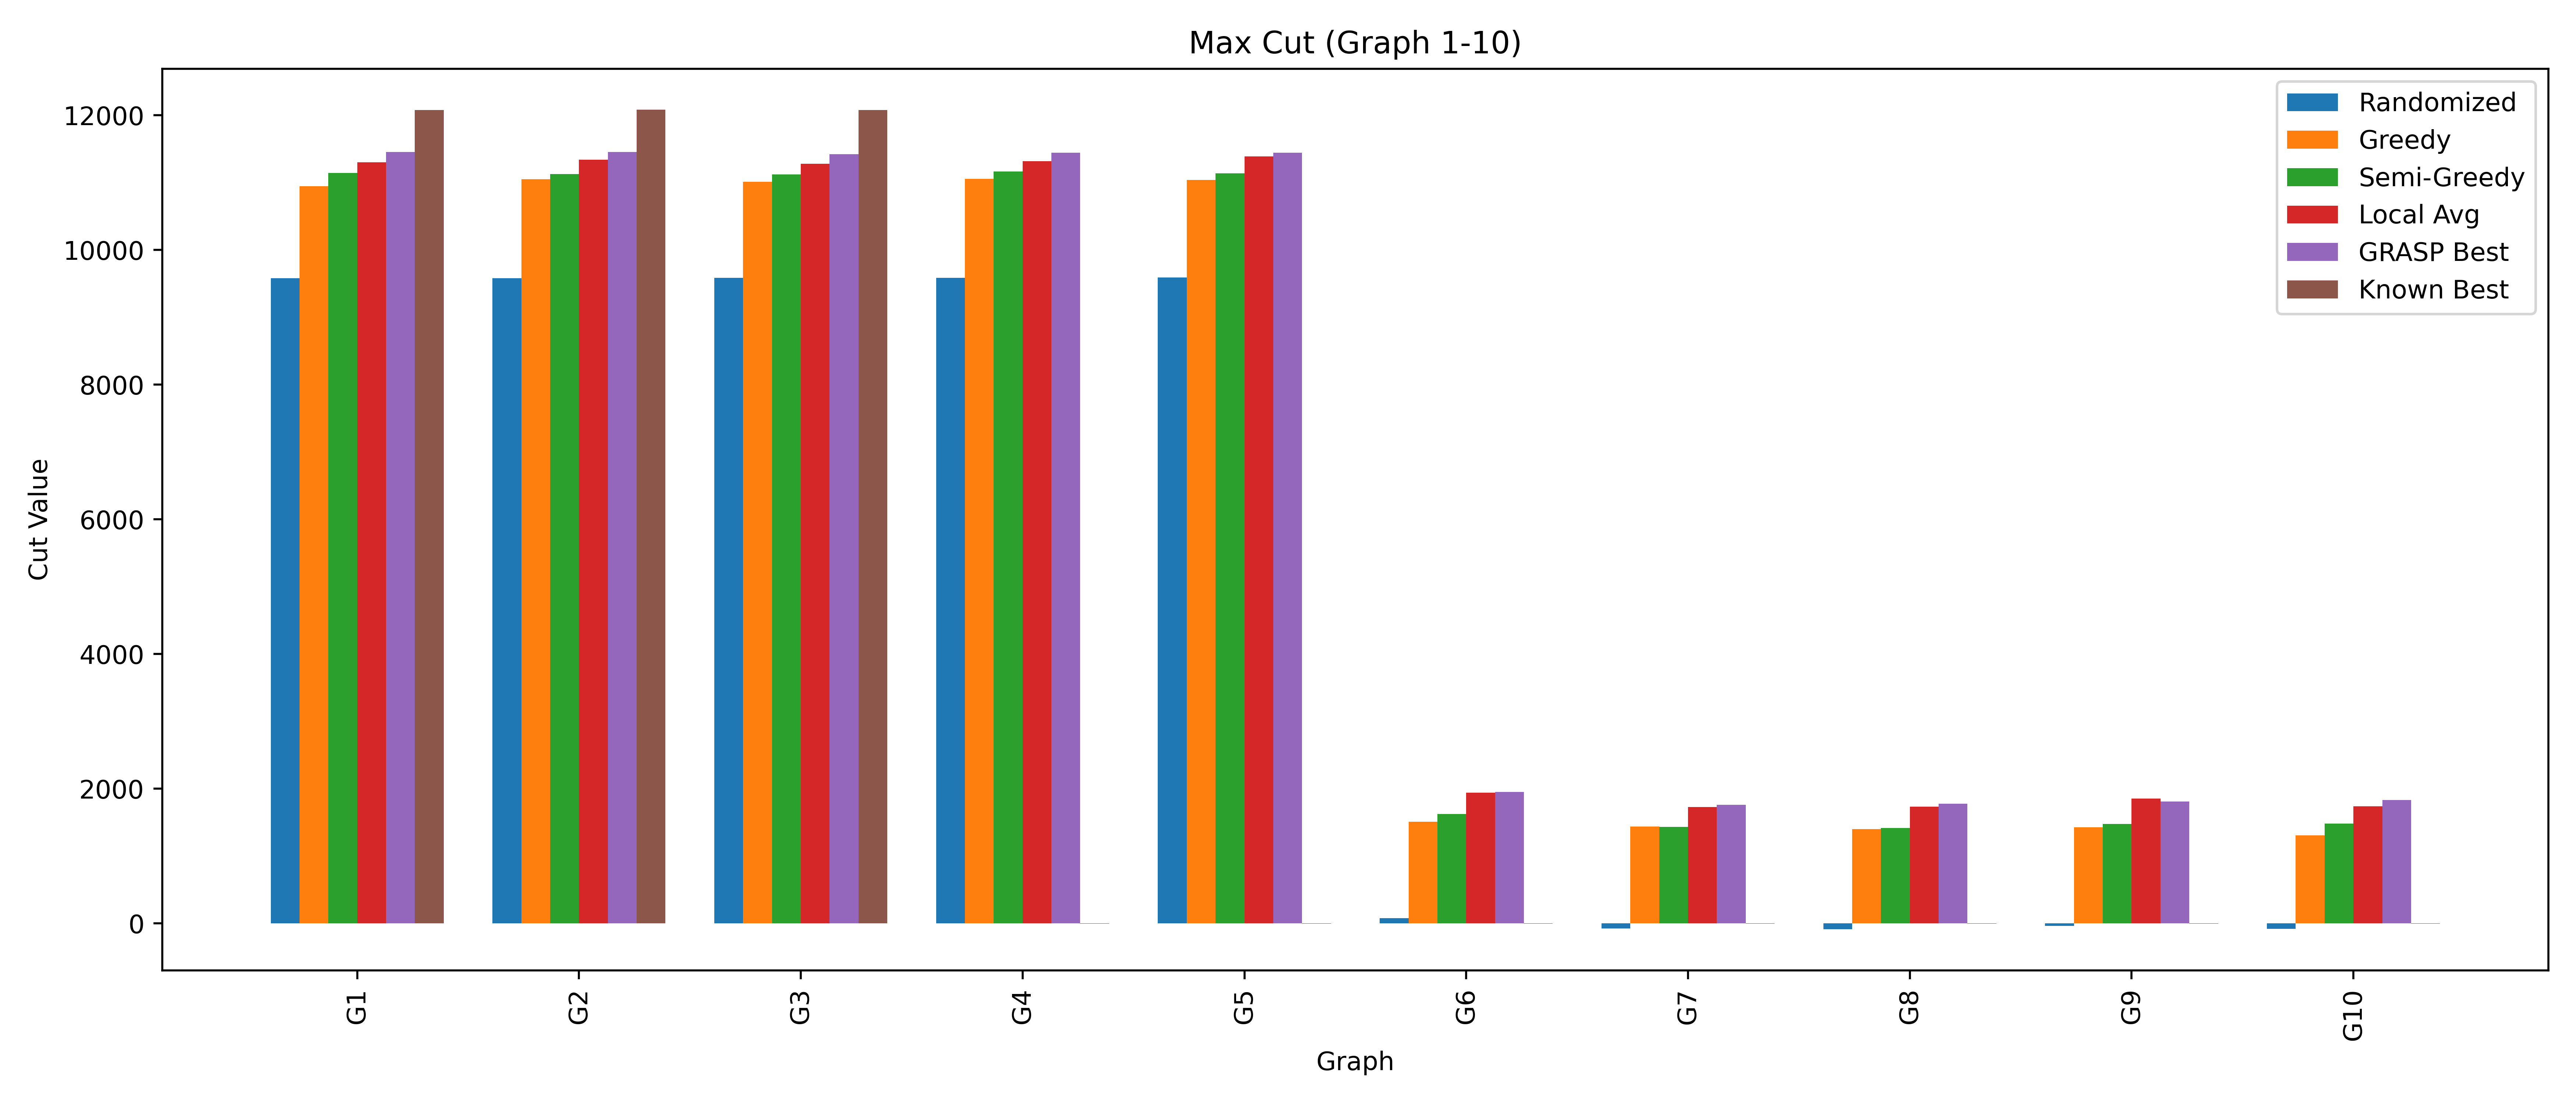
\includegraphics[width=0.95\textwidth]{../comparison_plot.png}
\end{center}

\section*{5. Additional Notes and Observations}
\begin{itemize}
    \item In most graphs, Greedy and Semi-Greedy produce close results, but Semi-Greedy slightly edges out due to randomization.
    \item Local search greatly improves solutions when initialized from Greedy or Semi-Greedy.
    \item GRASP consistently improves upon both, especially in denser graphs.
    \item Randomized solutions vary greatly; useful for baseline or stress-testing other heuristics.
    \item Execution time scales with graph size and number of iterations. GRASP's performance/quality tradeoff is tunable.
\end{itemize}

\section*{6. Conclusion}
GRASP, by combining diversification (through semi-greedy construction) and intensification (through local search), consistently yields high-quality solutions to the MAX-CUT problem. While more computationally intensive than simpler approaches, it provides the best trade-off between solution quality and runtime for many practical applications. The experimental results demonstrate that the additional computational effort is justified by the significant improvements in solution quality.

\end{document}
